\documentclass[12pt]{article}
\usepackage[T2A]{fontenc}
\usepackage[utf8]{inputenc}
\usepackage{multirow}
\usepackage{caption}
\usepackage{subcaption}
\usepackage{amsmath}
\usepackage{changepage}
\usepackage{graphicx}
\usepackage{float}
\usepackage[english,russian]{babel}
\usepackage{amsmath, amsfonts, amssymb, amsthm, mathtools}
\usepackage{xcolor}
\usepackage{array}
\usepackage{hyperref}
\usepackage[top = 1.5cm, left = 1.5 cm, right = 1.5 cm, bottom = 3 cm]{geometry}
\graphicspath{ {./images/} }
 
\title{Определение нагрева пули при попадании в мишень}
\author{Шахматов Андрей, Б02-304}
\date{\today}
  
\begin{document}
\begin{titlepage}
    \begin{center}
        {\large МОСКОВСКИЙ ФИЗИКО-ТЕХНИЧЕСКИЙ ИНСТИТУТ (НАЦИОНАЛЬНЫЙ ИССЛЕДОВАТЕЛЬСКИЙ УНИВЕРСИТЕТ)}
    \end{center}
    \begin{center}
        {\large Физтех-школа физики и исследований им. Ландау}
    \end{center}
    
    
    \vspace{3cm}
    {\huge
        \begin{center}
            \textbf{Определение нагрева пули при поражении цели}
        \end{center}
    }
    \vspace{2cm}
    \begin{flushright}
        {\LARGE Автор:\\ Шахматов Андрей Юрьевич \\
            \vspace{0.2cm}
            Б02-304}
    \end{flushright}
    \vspace{7 cm}
    \begin{center}
        Долгопрудный 2023
    \end{center}
\end{titlepage}

% \maketitle

\begin{abstract}
    Найдена начальная скорость пули при выстреле из духового ружья при помощи баллистических маятников, 
    принцип работы которых основан на вращательном и поступательном движении. Оценена теплота, выделяющаяся при столкновении пули с мишенью. 
    Найдено повышение температуры пули при столкновении с мишенью.
\end{abstract}

\tableofcontents

\section{Введение}
В современном военном и спортивном стрелковом деле одной из ключевых проблем является сохранение поражающей способности пуль 
во время их столкновения с мишенью. При попадании в мишень пуля испытывает значительные механические и термические нагрузки, 
которые могут привести к ее деформации и, следовательно, снижению поражающей способности. Однако, определение температуры, 
на которую нагревается пуля при столкновении с мишенью, позволит подобрать более термостабильные материалы для производства пуль.
Цель настоящей работы заключается в определении температуры нагрева пули при попадании в мишень.

\section{Методика}
Повышение температуры пули возможно оценить, считая, что вся теплота $Q$, выделившаяся при столкновении пошла на её нагрев. Тогда повышение 
температуры $t$ выражается через удельную теплоёмкость материала пули (свинца) $c = 140$ $\frac{\textrm{Дж}}{\textrm{кг}\cdot\textrm{°С}}$ 
и массу пули $m$
\begin{equation}\label{eq:1}
    t = \frac{Q}{cm}.
\end{equation}
При столкновении пули с баллистическим маятником теплота $Q$ выражается через начальную энегрию пули $E_0$, длину подвеса маятника $L$ и 
момент инерции матника $I$
\begin{equation}\label{eq:2}
    Q = E_0\left(1 - \frac{mL^2}{I}\right).
\end{equation}
Тогда задача сводится к нахождению начальной скорости пули $V$ и энергии $E_0 = \frac{mV^2}{2}$.
Начальную скорость пули можно найти анализируя максимальную амплитуду баллистического маятника после столкновения. Предложено два метода определении
начальной скорости пули: с использованием маятника A (Рис. \ref{fig:1}) и крутильного матяника B (Рис. \ref{fig:2}). Для маятника A, 
согласно \cite{LabBook}, скорость пули $V$ выражается через линейную амплитуду $A$, массу пули $m$, массу маятника $M$, длину подвеса $L$
\begin{equation}\label{eq:3}
    V = \frac{M}{m}\sqrt{\frac{g}{L}}A.
\end{equation}
В случае маятника B первоначально следует найти характерную величину $p = \sqrt{kI}$, где $k$ - крутильная жесткость маятника, $I$ - момент 
инерции маятника. Величину $p$ можно определить, измерив период колебаний маятника $T_2$ с дополнительными грузами массой $M$ и период колебаний
$T_1$ без них. Тогда величина $p$ выражается как
\begin{equation}\label{eq:4}
    p = \frac{4 \pi MR^2 T_1}{T_1^2 - T_2^2},
\end{equation}
где $R$ - расстояние от оси вращения до грузов массой $M$. Тогда начальная скорость пули выражается через параметр $p$, линейную амплитуду 
колебаний $A$, расстояние до точки измерения амплитуды $l$, массу пули $m$ и расстояние от оси вращения до мишени $r$:
\begin{equation}\label{eq:5}
    V = \frac{A}{l} \frac{p}{mr}.
\end{equation}

\begin{figure}
    \begin{center}
        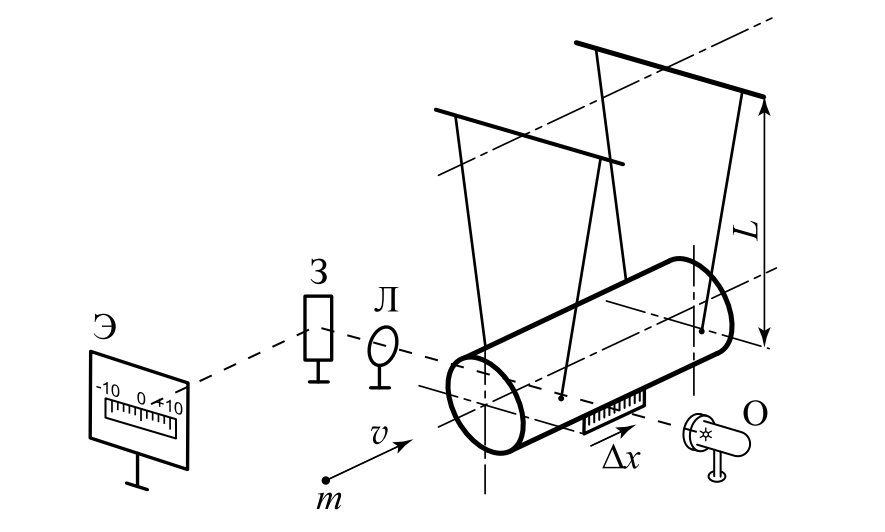
\includegraphics[width=0.5\textwidth]{im1.png}
    \end{center}
    \caption{Схема экспериментальной установки по измерению начальной скорости пули с помощью маятника, основанного на поступательном движении}
    \label{fig:1}
\end{figure}
\begin{figure}
    \begin{center}
        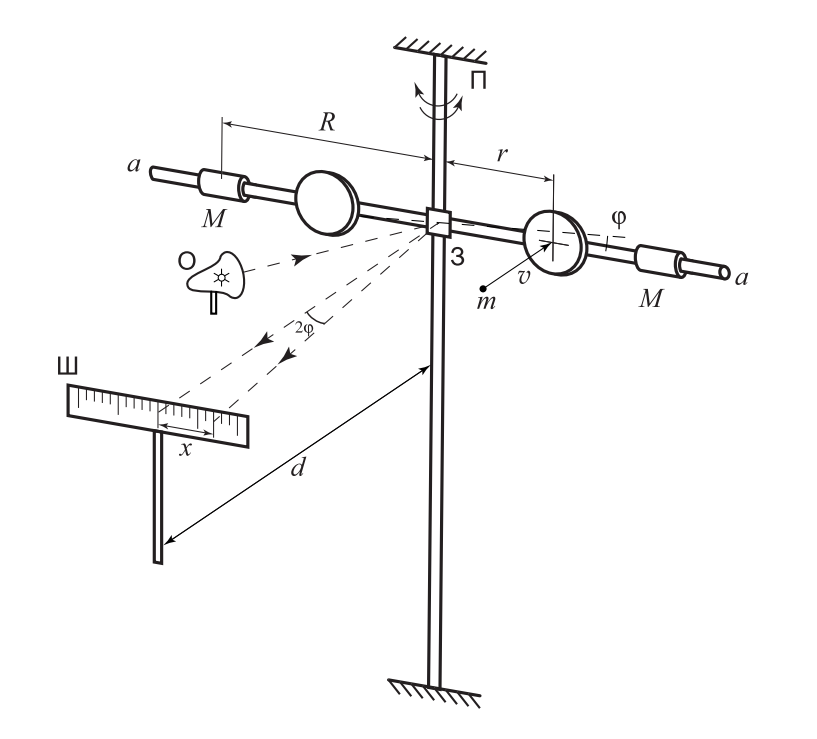
\includegraphics[width=0.5\textwidth]{im2.png}
    \end{center}
    \caption{Схема экспериментальной установки по измерению начальной скорости пули с помощью крутильного маятника}
    \label{fig:2}
\end{figure}
\section{Результаты и их анализ}
С использованием линейки и весов измерены параметры маятника B (Таблица \ref{tab:1}) и маятника A (Таблица \ref{tab:2}).
Найдены периоды колебаний крутильного маятника с грузами $T_1 = 6.683 \pm 0.018$ с и без грузов $T_2 = 4.993 \pm 0.018$ с. 
С использованием выражения \ref{eq:4} найдено значение параметра $p = 0.403 \pm 0.010$ $\frac{\textrm{кг}\cdot\textrm{м}^2}{\textrm{с}}$.
Измерены массы 10 пуль. Для первых 5 пуль проведены измерения амплитуды на маятнике A (Таблица \ref{tab:3}). С использованием 
выражения \ref{eq:3} найдена начальная скорость пуль (Таблица \ref{tab:5}). Для оставшийхся 5 пуль проведены измерения амплитуды на маятнике B
 (Таблица \ref{tab:4}). С использованием выражения \ref{eq:5} найдена начальная скорость пуль (Таблица \ref{tab:5}).
\begin{table}[H]
    \centering
    \begin{tabular}{|r|r|r|r|r|r|}
        \hline
        \multicolumn{3}{|c|}{Маятник A} & 
        \multicolumn{3}{|c|}{Маятник B}                                                                                                                                                \\
        \hline
        $m$, г                                       & $u$, $\frac{\textrm{м}}{\textrm{с}} \cdot 10^2$ & $\epsilon_u$ & $m$, г & $u$, $\frac{\textrm{м}}{\textrm{с}} \cdot 10^2$ & $\epsilon_u$ \\
        \hline
        0.5097                                       & 1.35                                            & 0.02         & 0.5068 & 1.63                                            & 0.03         \\
        0.5047                                       & 1.36                                            & 0.02         & 0.5067 & 1.58                                            & 0.03         \\
        0.5037                                       & 1.36                                            & 0.02         & 0.5124 & 1.62                                            & 0.03         \\
        0.5046                                       & 1.39                                            & 0.02         & 0.5007 & 1.71                                            & 0.03         \\
        0.5103                                       & 1.37                                            & 0.02         & 0.5063 & 1.64                                            & 0.03         \\
        \hline
    \end{tabular}
    
    \caption{Начальные скорости пуль на маятниках A и B. $m$ - масса пули, $u$ - начальная скорость пули,
        $\epsilon_u$ - относительная погрешность $u$.}
    \label{tab:5}
\end{table}
Для определения теплоты, которая выделилась при столкновении, были использованы результаты, полученные с использованием маятника A.
Используя выражения \ref{eq:1} и \ref{eq:2} рассчитаны теплота, выделившаяся при столкновении, и повышение температуры пули при условии, что вся
выделившаяся теплота пошла на её нагрев (Таблица \ref{tab:6}).
\begin{table}[H]
    \centering
    \begin{tabular}{|r|r|r|}
        \hline
        $m$, г & $Q$, Дж & $t$, \textcelsius \\
        \hline
        0.5097 & 4.63    & 64.9              \\
        0.5047 & 4.68    & 66.0              \\
        0.5037 & 4.68    & 66.0              \\
        0.5046 & 4.89    & 69.0              \\
        0.5103 & 4.83    & 68.0              \\
        \hline
    \end{tabular}
    \caption{Теплоты $Q$, выделившиеся при столконовении, и повышения температур пуль $t$.
        Относительная погрешность $\epsilon_Q = 0.04$, относительная погрешность $\epsilon_t = 0.04$.}
    \label{tab:6}
\end{table}
Средняя температура нагрева пуль оказалась равна $t = 66.9 \pm 1.3$, \textcelsius. Принимая 
температуру плавления свинца за $T = 327.46$ \textcelsius  и начальную температуру пули $t_0 = 20$ \textcelsius, можно сделать вывод о том, что
энергии, сообщаемой пули при выстреле из духовой винтовки недостаточно, чтобы пуля расплавилась при попадании в мишень, так как $T$ меньше 
чем $t_0 + t$ чуть менее чем в четыре раза.

\section{Выводы}
В среденем скорость вылета пули из духового ружья составила $u = 1.37 \pm 0.27 \cdot 10^{2}$ $\frac{\textrm{м}}{\textrm{с}}$. С учётом
данной начальной скорости вылета пули была получена оценка теплоты, выделяющейся при столкновении пули с мишенью $Q = 4.74 \pm 0.10$ Дж.
Средняя температура нагрева пули при столкновении с мишенью оказалась равна $t = 66.9 \pm 1.3$ \textcelsius.

\section{Использованная литература}
\begin{thebibliography}{9}
    \bibitem{LabBook}
    Лабораторный практикум по общей физике, Том 1, под редакцией А. Д. Гладуна
\end{thebibliography}

\section{Приложения}
\subsection{Данные результатов измерений геометрических и физических характеристик маятников} \label{app_1}
\begin{table}[H]
    \centering
    \begin{tabular}{|l|l|l|l|l|l|l|l|l|}
        \hline
                    & $m_1$, кг & $m_2$, кг & $M$, кг & $R$, м & $r$, м & $l$, м \\ 
        \hline
        Измерения   & 0.7306    & 0.7299    & 1.4605  & 0.360  & 0.204  & 1.430  \\
        Погрешности & 0.0001    & 0.0001    & 0.0001  & 0.005  & 0.005  & 0.005  \\
        \hline
    \end{tabular}
    
    \caption{Характеристики маятника B. $m_1$ - масса дополнительного груза с одной стороны,
        $m_2$ - масса дополнительного груза с другой стороны, $M$ - суммарная масса дополнительных грузов, $R$ - расстояние от оси вращения до
        точки подвеса дополнительных грузов, $r$ - расстояние от оси вращения до мишени, $l$ - расстояние от оси вращения до точки измерения амплитуды.}
    \label{tab:1}
\end{table}

\begin{table}[H]
    \centering
    \begin{tabular}{|l|l|l|l|l|l|l|l|l|}
        \hline
                    & $M$, кг & $L$, м \\ 
        \hline
        Измерения   & 2.900   & 2.210  \\
        Погрешности & 0.005   & 0.005  \\
        \hline
    \end{tabular}
    
    \caption{Характеристики маятника А. $M$ - масса маятника, $L$ - расстояние от точки подвеса до маятника.}
    \label{tab:2}
\end{table}
\subsection{Результаты измерений амплитуд колебаний маятников} \label{app_2}
Диаметр пули $d = 4.5 \pm 0.1$ см.
\begin{table}[H]
    \centering
    \begin{tabular}{|r|r|}
        \hline
        $m$, г & $A$, см \\
        \hline
        0.5097 & 11.25   \\
        0.5047 & 11.25   \\
        0.5037 & 11.25   \\
        0.5046 & 11.50   \\
        0.5103 & 11.50   \\
        \hline
    \end{tabular}
    \caption{Массы пуль $m$ и линейные амплитуды отклонения $A$, измеренные на матянике B.}
    \label{tab:3}
\end{table}

\begin{table}[H]
    \centering
    \begin{tabular}{|r|r|}
        \hline
        $m$, г & $A$, см \\
        \hline
        0.5068 & 6.0     \\
        0.5067 & 5.8     \\
        0.5124 & 6.0     \\
        0.5007 & 6.2     \\
        0.5063 & 6.0     \\
        \hline
    \end{tabular}
    \caption{Массы пуль $m$ и линейные амплитуды отклонения $A$, измеренные на матянике B.}
    \label{tab:4}
\end{table}
\end{document}